% Created by tikzDevice version 0.12.6 on 2024-11-13 12:23:55
% !TEX encoding = UTF-8 Unicode
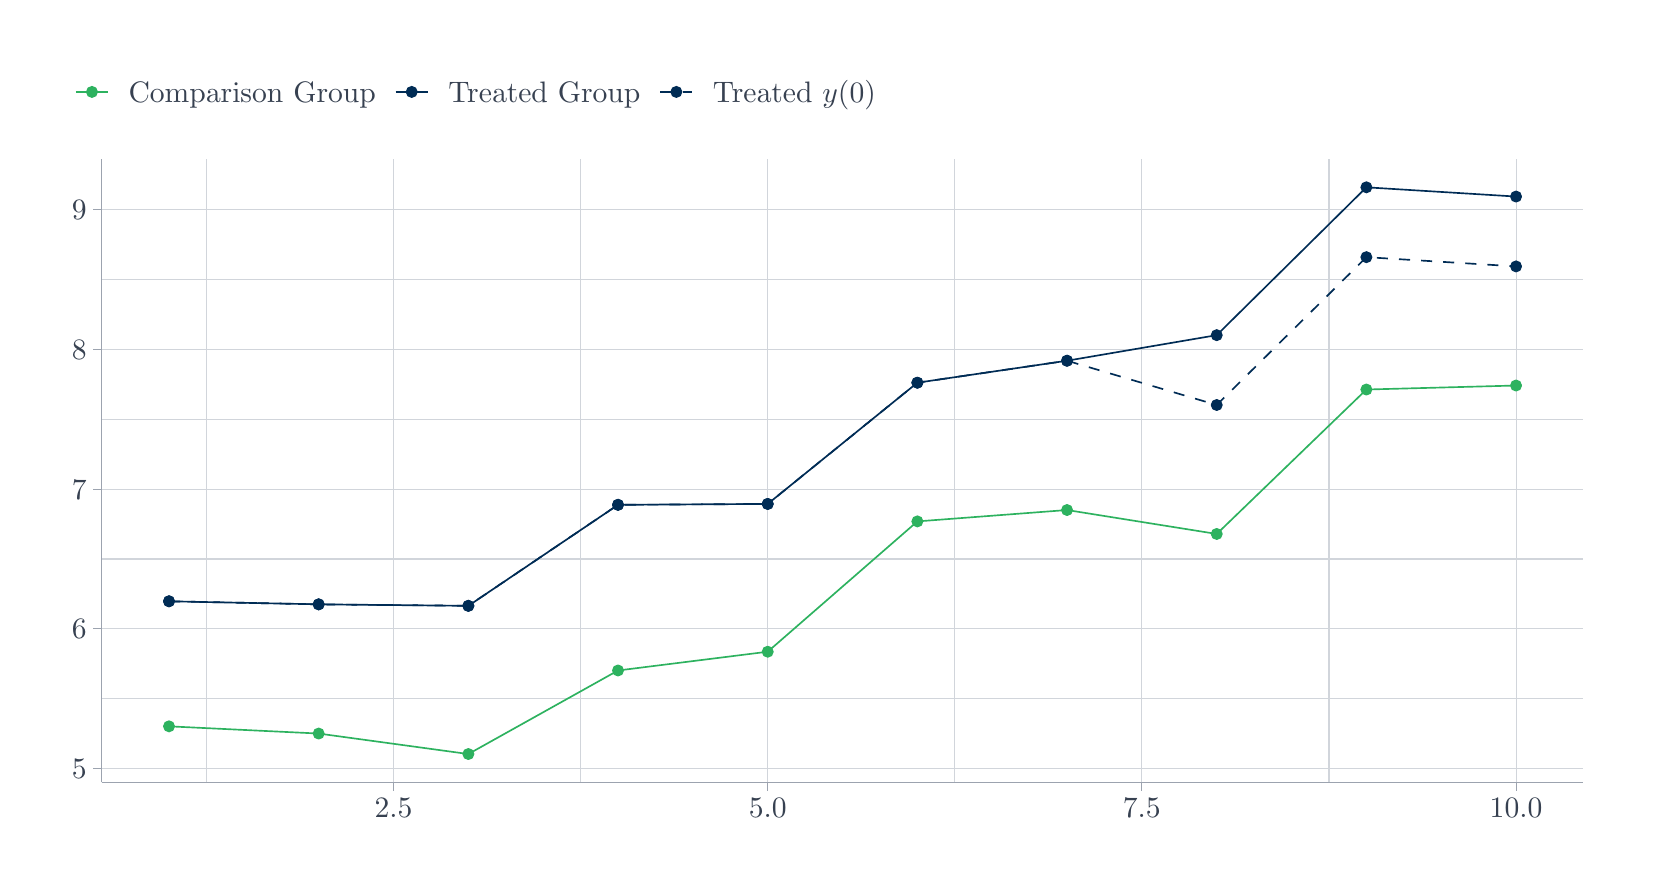
\begin{tikzpicture}[x=1pt,y=1pt]
\definecolor{fillColor}{RGB}{255,255,255}
\path[use as bounding box,fill=fillColor] (0,0) rectangle (578.16,303.53);
\begin{scope}
\path[clip] (  0.00,  0.00) rectangle (578.16,303.53);
\definecolor{drawColor}{RGB}{255,255,255}

\path[draw=drawColor,line width= 0.6pt,line join=round,line cap=round,fill=fillColor] (  0.00,  0.00) rectangle (578.16,303.53);
\end{scope}
\begin{scope}
\path[clip] ( 26.73, 30.82) rectangle (562.16,256.08);
\definecolor{drawColor}{RGB}{255,255,255}
\definecolor{fillColor}{RGB}{255,255,255}

\path[draw=drawColor,line width= 0.6pt,line join=round,line cap=round,fill=fillColor] ( 26.73, 30.82) rectangle (562.16,256.08);
\definecolor{drawColor}{RGB}{209,213,219}

\path[draw=drawColor,line width= 0.4pt,line join=round] ( 26.73, 61.07) --
	(562.16, 61.07);

\path[draw=drawColor,line width= 0.4pt,line join=round] ( 26.73,111.55) --
	(562.16,111.55);

\path[draw=drawColor,line width= 0.4pt,line join=round] ( 26.73,162.02) --
	(562.16,162.02);

\path[draw=drawColor,line width= 0.4pt,line join=round] ( 26.73,212.50) --
	(562.16,212.50);

\path[draw=drawColor,line width= 0.4pt,line join=round] ( 64.59, 30.82) --
	( 64.59,256.08);

\path[draw=drawColor,line width= 0.4pt,line join=round] (199.80, 30.82) --
	(199.80,256.08);

\path[draw=drawColor,line width= 0.4pt,line join=round] (335.01, 30.82) --
	(335.01,256.08);

\path[draw=drawColor,line width= 0.4pt,line join=round] (470.22, 30.82) --
	(470.22,256.08);

\path[draw=drawColor,line width= 0.4pt,line join=round] ( 26.73, 35.83) --
	(562.16, 35.83);

\path[draw=drawColor,line width= 0.4pt,line join=round] ( 26.73, 86.31) --
	(562.16, 86.31);

\path[draw=drawColor,line width= 0.4pt,line join=round] ( 26.73,136.78) --
	(562.16,136.78);

\path[draw=drawColor,line width= 0.4pt,line join=round] ( 26.73,187.26) --
	(562.16,187.26);

\path[draw=drawColor,line width= 0.4pt,line join=round] ( 26.73,237.74) --
	(562.16,237.74);

\path[draw=drawColor,line width= 0.4pt,line join=round] (132.20, 30.82) --
	(132.20,256.08);

\path[draw=drawColor,line width= 0.4pt,line join=round] (267.41, 30.82) --
	(267.41,256.08);

\path[draw=drawColor,line width= 0.4pt,line join=round] (402.61, 30.82) --
	(402.61,256.08);

\path[draw=drawColor,line width= 0.4pt,line join=round] (537.82, 30.82) --
	(537.82,256.08);
\definecolor{drawColor}{RGB}{45,178,95}

\path[draw=drawColor,line width= 0.6pt,line join=round] ( 51.07, 51.07) --
	(105.15, 48.46) --
	(159.24, 41.06) --
	(213.32, 71.25) --
	(267.41, 78.03) --
	(321.49,125.12) --
	(375.57,129.23) --
	(429.66,120.58) --
	(483.74,172.77) --
	(537.82,174.22);
\definecolor{fillColor}{RGB}{45,178,95}

\path[draw=drawColor,line width= 0.4pt,line join=round,line cap=round,fill=fillColor] ( 51.07, 51.07) circle (  1.96);

\path[draw=drawColor,line width= 0.4pt,line join=round,line cap=round,fill=fillColor] (105.15, 48.46) circle (  1.96);

\path[draw=drawColor,line width= 0.4pt,line join=round,line cap=round,fill=fillColor] (159.24, 41.06) circle (  1.96);

\path[draw=drawColor,line width= 0.4pt,line join=round,line cap=round,fill=fillColor] (213.32, 71.25) circle (  1.96);

\path[draw=drawColor,line width= 0.4pt,line join=round,line cap=round,fill=fillColor] (267.41, 78.03) circle (  1.96);

\path[draw=drawColor,line width= 0.4pt,line join=round,line cap=round,fill=fillColor] (321.49,125.12) circle (  1.96);

\path[draw=drawColor,line width= 0.4pt,line join=round,line cap=round,fill=fillColor] (375.57,129.23) circle (  1.96);

\path[draw=drawColor,line width= 0.4pt,line join=round,line cap=round,fill=fillColor] (429.66,120.58) circle (  1.96);

\path[draw=drawColor,line width= 0.4pt,line join=round,line cap=round,fill=fillColor] (483.74,172.77) circle (  1.96);

\path[draw=drawColor,line width= 0.4pt,line join=round,line cap=round,fill=fillColor] (537.82,174.22) circle (  1.96);
\definecolor{drawColor}{RGB}{0,44,85}

\path[draw=drawColor,line width= 0.6pt,line join=round] ( 51.07, 96.25) --
	(105.15, 95.15) --
	(159.24, 94.61) --
	(213.32,131.11) --
	(267.41,131.43) --
	(321.49,175.24) --
	(375.57,183.18) --
	(429.66,192.42) --
	(483.74,245.84) --
	(537.82,242.50);
\definecolor{fillColor}{RGB}{0,44,85}

\path[draw=drawColor,line width= 0.4pt,line join=round,line cap=round,fill=fillColor] ( 51.07, 96.25) circle (  1.96);

\path[draw=drawColor,line width= 0.4pt,line join=round,line cap=round,fill=fillColor] (105.15, 95.15) circle (  1.96);

\path[draw=drawColor,line width= 0.4pt,line join=round,line cap=round,fill=fillColor] (159.24, 94.61) circle (  1.96);

\path[draw=drawColor,line width= 0.4pt,line join=round,line cap=round,fill=fillColor] (213.32,131.11) circle (  1.96);

\path[draw=drawColor,line width= 0.4pt,line join=round,line cap=round,fill=fillColor] (267.41,131.43) circle (  1.96);

\path[draw=drawColor,line width= 0.4pt,line join=round,line cap=round,fill=fillColor] (321.49,175.24) circle (  1.96);

\path[draw=drawColor,line width= 0.4pt,line join=round,line cap=round,fill=fillColor] (375.57,183.18) circle (  1.96);

\path[draw=drawColor,line width= 0.4pt,line join=round,line cap=round,fill=fillColor] (429.66,192.42) circle (  1.96);

\path[draw=drawColor,line width= 0.4pt,line join=round,line cap=round,fill=fillColor] (483.74,245.84) circle (  1.96);

\path[draw=drawColor,line width= 0.4pt,line join=round,line cap=round,fill=fillColor] (537.82,242.50) circle (  1.96);

\path[draw=drawColor,line width= 0.6pt,dash pattern=on 4pt off 4pt ,line join=round] ( 51.07, 96.25) --
	(105.15, 95.15) --
	(159.24, 94.61) --
	(213.32,131.11) --
	(267.41,131.43) --
	(321.49,175.24) --
	(375.57,183.18) --
	(429.66,167.18) --
	(483.74,220.60) --
	(537.82,217.26);

\path[draw=drawColor,line width= 0.4pt,line join=round,line cap=round,fill=fillColor] ( 51.07, 96.25) circle (  1.96);

\path[draw=drawColor,line width= 0.4pt,line join=round,line cap=round,fill=fillColor] (105.15, 95.15) circle (  1.96);

\path[draw=drawColor,line width= 0.4pt,line join=round,line cap=round,fill=fillColor] (159.24, 94.61) circle (  1.96);

\path[draw=drawColor,line width= 0.4pt,line join=round,line cap=round,fill=fillColor] (213.32,131.11) circle (  1.96);

\path[draw=drawColor,line width= 0.4pt,line join=round,line cap=round,fill=fillColor] (267.41,131.43) circle (  1.96);

\path[draw=drawColor,line width= 0.4pt,line join=round,line cap=round,fill=fillColor] (321.49,175.24) circle (  1.96);

\path[draw=drawColor,line width= 0.4pt,line join=round,line cap=round,fill=fillColor] (375.57,183.18) circle (  1.96);

\path[draw=drawColor,line width= 0.4pt,line join=round,line cap=round,fill=fillColor] (429.66,167.18) circle (  1.96);

\path[draw=drawColor,line width= 0.4pt,line join=round,line cap=round,fill=fillColor] (483.74,220.60) circle (  1.96);

\path[draw=drawColor,line width= 0.4pt,line join=round,line cap=round,fill=fillColor] (537.82,217.26) circle (  1.96);
\end{scope}
\begin{scope}
\path[clip] (  0.00,  0.00) rectangle (578.16,303.53);
\definecolor{drawColor}{RGB}{156,163,175}

\path[draw=drawColor,line width= 0.3pt,line join=round] ( 26.73, 30.82) --
	( 26.73,256.08);
\end{scope}
\begin{scope}
\path[clip] (  0.00,  0.00) rectangle (578.16,303.53);
\definecolor{drawColor}{RGB}{55,65,81}

\node[text=drawColor,anchor=base east,inner sep=0pt, outer sep=0pt, scale=  1.07] at ( 21.33, 32.16) {5};

\node[text=drawColor,anchor=base east,inner sep=0pt, outer sep=0pt, scale=  1.07] at ( 21.33, 82.63) {6};

\node[text=drawColor,anchor=base east,inner sep=0pt, outer sep=0pt, scale=  1.07] at ( 21.33,133.11) {7};

\node[text=drawColor,anchor=base east,inner sep=0pt, outer sep=0pt, scale=  1.07] at ( 21.33,183.59) {8};

\node[text=drawColor,anchor=base east,inner sep=0pt, outer sep=0pt, scale=  1.07] at ( 21.33,234.06) {9};
\end{scope}
\begin{scope}
\path[clip] (  0.00,  0.00) rectangle (578.16,303.53);
\definecolor{drawColor}{RGB}{156,163,175}

\path[draw=drawColor,line width= 0.3pt,line join=round] ( 23.73, 35.83) --
	( 26.73, 35.83);

\path[draw=drawColor,line width= 0.3pt,line join=round] ( 23.73, 86.31) --
	( 26.73, 86.31);

\path[draw=drawColor,line width= 0.3pt,line join=round] ( 23.73,136.78) --
	( 26.73,136.78);

\path[draw=drawColor,line width= 0.3pt,line join=round] ( 23.73,187.26) --
	( 26.73,187.26);

\path[draw=drawColor,line width= 0.3pt,line join=round] ( 23.73,237.74) --
	( 26.73,237.74);
\end{scope}
\begin{scope}
\path[clip] (  0.00,  0.00) rectangle (578.16,303.53);
\definecolor{drawColor}{RGB}{156,163,175}

\path[draw=drawColor,line width= 0.3pt,line join=round] ( 26.73, 30.82) --
	(562.16, 30.82);
\end{scope}
\begin{scope}
\path[clip] (  0.00,  0.00) rectangle (578.16,303.53);
\definecolor{drawColor}{RGB}{156,163,175}

\path[draw=drawColor,line width= 0.3pt,line join=round] (132.20, 27.82) --
	(132.20, 30.82);

\path[draw=drawColor,line width= 0.3pt,line join=round] (267.41, 27.82) --
	(267.41, 30.82);

\path[draw=drawColor,line width= 0.3pt,line join=round] (402.61, 27.82) --
	(402.61, 30.82);

\path[draw=drawColor,line width= 0.3pt,line join=round] (537.82, 27.82) --
	(537.82, 30.82);
\end{scope}
\begin{scope}
\path[clip] (  0.00,  0.00) rectangle (578.16,303.53);
\definecolor{drawColor}{RGB}{55,65,81}

\node[text=drawColor,anchor=base,inner sep=0pt, outer sep=0pt, scale=  1.07] at (132.20, 18.07) {2.5};

\node[text=drawColor,anchor=base,inner sep=0pt, outer sep=0pt, scale=  1.07] at (267.41, 18.07) {5.0};

\node[text=drawColor,anchor=base,inner sep=0pt, outer sep=0pt, scale=  1.07] at (402.61, 18.07) {7.5};

\node[text=drawColor,anchor=base,inner sep=0pt, outer sep=0pt, scale=  1.07] at (537.82, 18.07) {10.0};
\end{scope}
\begin{scope}
\path[clip] (  0.00,  0.00) rectangle (578.16,303.53);
\definecolor{drawColor}{RGB}{255,255,255}
\definecolor{fillColor}{RGB}{255,255,255}

\path[draw=drawColor,line width= 0.6pt,line join=round,line cap=round,fill=fillColor] ( 16.00,268.08) rectangle (306.31,287.53);
\end{scope}
\begin{scope}
\path[clip] (  0.00,  0.00) rectangle (578.16,303.53);
\definecolor{drawColor}{RGB}{255,255,255}
\definecolor{fillColor}{RGB}{255,255,255}

\path[draw=drawColor,line width= 0.6pt,line join=round,line cap=round,fill=fillColor] ( 16.00,273.08) rectangle ( 30.45,287.53);
\end{scope}
\begin{scope}
\path[clip] (  0.00,  0.00) rectangle (578.16,303.53);
\definecolor{drawColor}{RGB}{45,178,95}

\path[draw=drawColor,line width= 0.6pt,line join=round] ( 17.45,280.31) -- ( 29.01,280.31);
\end{scope}
\begin{scope}
\path[clip] (  0.00,  0.00) rectangle (578.16,303.53);
\definecolor{drawColor}{RGB}{45,178,95}
\definecolor{fillColor}{RGB}{45,178,95}

\path[draw=drawColor,line width= 0.4pt,line join=round,line cap=round,fill=fillColor] ( 23.23,280.31) circle (  1.96);
\end{scope}
\begin{scope}
\path[clip] (  0.00,  0.00) rectangle (578.16,303.53);
\definecolor{drawColor}{RGB}{255,255,255}
\definecolor{fillColor}{RGB}{255,255,255}

\path[draw=drawColor,line width= 0.6pt,line join=round,line cap=round,fill=fillColor] (131.54,273.08) rectangle (146.00,287.53);
\end{scope}
\begin{scope}
\path[clip] (  0.00,  0.00) rectangle (578.16,303.53);
\definecolor{drawColor}{RGB}{0,44,85}

\path[draw=drawColor,line width= 0.6pt,line join=round] (132.99,280.31) -- (144.55,280.31);
\end{scope}
\begin{scope}
\path[clip] (  0.00,  0.00) rectangle (578.16,303.53);
\definecolor{drawColor}{RGB}{0,44,85}
\definecolor{fillColor}{RGB}{0,44,85}

\path[draw=drawColor,line width= 0.4pt,line join=round,line cap=round,fill=fillColor] (138.77,280.31) circle (  1.96);
\end{scope}
\begin{scope}
\path[clip] (  0.00,  0.00) rectangle (578.16,303.53);
\definecolor{drawColor}{RGB}{255,255,255}
\definecolor{fillColor}{RGB}{255,255,255}

\path[draw=drawColor,line width= 0.6pt,line join=round,line cap=round,fill=fillColor] (227.17,273.08) rectangle (241.62,287.53);
\end{scope}
\begin{scope}
\path[clip] (  0.00,  0.00) rectangle (578.16,303.53);
\definecolor{drawColor}{RGB}{0,44,85}

\path[draw=drawColor,line width= 0.6pt,dash pattern=on 4pt off 4pt ,line join=round] (228.62,280.31) -- (240.18,280.31);
\end{scope}
\begin{scope}
\path[clip] (  0.00,  0.00) rectangle (578.16,303.53);
\definecolor{drawColor}{RGB}{0,44,85}
\definecolor{fillColor}{RGB}{0,44,85}

\path[draw=drawColor,line width= 0.4pt,line join=round,line cap=round,fill=fillColor] (234.40,280.31) circle (  1.96);
\end{scope}
\begin{scope}
\path[clip] (  0.00,  0.00) rectangle (578.16,303.53);
\definecolor{drawColor}{RGB}{55,65,81}

\node[text=drawColor,anchor=base west,inner sep=0pt, outer sep=0pt, scale=  1.07] at ( 36.45,276.63) {Comparison Group};
\end{scope}
\begin{scope}
\path[clip] (  0.00,  0.00) rectangle (578.16,303.53);
\definecolor{drawColor}{RGB}{55,65,81}

\node[text=drawColor,anchor=base west,inner sep=0pt, outer sep=0pt, scale=  1.07] at (152.00,276.63) {Treated Group};
\end{scope}
\begin{scope}
\path[clip] (  0.00,  0.00) rectangle (578.16,303.53);
\definecolor{drawColor}{RGB}{55,65,81}

\node[text=drawColor,anchor=base west,inner sep=0pt, outer sep=0pt, scale=  1.07] at (247.62,276.63) {Treated $y(0)$};
\end{scope}
\end{tikzpicture}
